\documentclass[a4paper,twoside]{article}
\usepackage{blindtext}  
\usepackage{geometry}

% Chinese support
\usepackage[UTF8, scheme = plain]{ctex}

% Page margin layout
\geometry{left=2.3cm,right=2cm,top=2.5cm,bottom=2.0cm}


\usepackage{listings}
\usepackage{xcolor}
\usepackage{geometry}
\usepackage{amsmath}
\usepackage{float}
\usepackage{hyperref}

\usepackage{graphics}
\usepackage{graphicx}
\usepackage{subcaption}
\usepackage{epsfig}
\usepackage{float}

\usepackage{algorithm}
\usepackage[noend]{algpseudocode}

\usepackage{booktabs}
\usepackage{threeparttable}
\usepackage{longtable}
\usepackage{tikz}
\usepackage{multicol}
\usepackage{pgfplots}
\pgfplotsset{compat=1.9}
\pgfplotsset{
    myplotstyle/.style={
    legend style={draw=none, font=\small},
    legend cell align=left,
    legend pos=north east,
    ylabel style={align=center, font=\bfseries\boldmath},
    xlabel style={align=center, font=\bfseries\boldmath},
    x tick label style={font=\bfseries\boldmath},
    y tick label style={font=\bfseries\boldmath},
    scaled ticks=false,
    every axis plot/.append style={thick},
    },
}

% cite package, to clean up citations in the main text. Do not remove.
\usepackage{cite}

\usepackage{color,xcolor}

%% The amssymb package provides various useful mathematical symbols
% \usepackage{amssymb}
%% The amsthm package provides extended theorem environments
% \usepackage{amsthm}
% \usepackage{amsfonts}
\usepackage{enumerate}
\usepackage{enumitem}
\usepackage{listings}
\usepackage{minted}


\usepackage{indentfirst}
\setlength{\parindent}{2em} % Make two letter space in the first paragraph
\usepackage{setspace}
\linespread{1.5} % Line spacing setting
\usepackage{siunitx}
\setlength{\parskip}{0.5em} % Paragraph spacing setting

% \usepackage[contents =22920202204622, scale = 10, color = black, angle = 50, opacity = .10]{background}

\renewcommand{\figurename}{图}
\renewcommand{\listingscaption}{代码}
\renewcommand{\tablename}{表格}
\renewcommand{\contentsname}{目录}
\floatname{algorithm}{算法}

\graphicspath{ {images/} }

%%%%%%%%%%%%%
\newcommand{\StudentNumber}{22920202204622}  % Fill your student number here
\newcommand{\StudentName}{熊恪峥}  % Replace your name here
\newcommand{\PaperTitle}{实验(四)}  % Change your paper title here
\newcommand{\PaperType}{实验报告} % Replace the type of your report here
\newcommand{\Date}{2023年5月18日}
\newcommand{\College}{信息学院}
\newcommand{\CourseName}{数据库}
%%%%%%%%%%%%%

%% Page header and footer setting
\usepackage{fancyhdr}
\usepackage{lastpage}
\pagestyle{fancy}
\fancyhf{}
% This requires the document to be twoside
\fancyhead[LO]{\texttt{\StudentName }}
\fancyhead[LE]{\texttt{\StudentNumber}}
\fancyhead[C]{\texttt{\PaperTitle }}
\fancyhead[R]{\texttt{第{\thepage}页,共\pageref*{LastPage}页}}


\title{\PaperTitle}
\author{\StudentName}
\date{\Date}

\algnewcommand\algorithmicinput{\textbf{Input:}}
\algnewcommand\algorithmicoutput{\textbf{Output:}}
\algnewcommand\Input{\item[\algorithmicinput]}%
\algnewcommand\Output{\item[\algorithmicoutput]}%

\usetikzlibrary{positioning, shapes.geometric}

\begin{document}
	
%%%%%%%%%%%%%%%%%%%%%%%%%%%%%%%%%%%%%%%%%%%%
\makeatletter % change default title style
\renewcommand*\maketitle{%
	\begin{center} 
		\bfseries  % title 
		{\LARGE \@title \par}  % LARGE typesetting
		\vskip 1em  %  margin 1em
		{\global\let\author\@empty}  % no author information
		{\global\let\date\@empty}  % no date
		\thispagestyle{empty}   %  empty page style
	\end{center}%
	\setcounter{footnote}{0}%
}
\makeatother
%%%%%%%%%%%%%%%%%%%%%%%%%%%%%%%%%%%%%%%%%%%%
	
	
\thispagestyle{empty}

\vspace*{1cm}

\begin{figure}[htb]
	\centering
	
\includegraphics[width=4.0cm]{logo.png}
\end{figure}

\vspace*{1cm}

\begin{center}
	\Huge{\textbf{\PaperType}}
	
	\Large{\PaperTitle}
\end{center}

\vspace*{1cm}

\begin{table}[h]
	\centering	
	\begin{Large}
		\renewcommand{\arraystretch}{1.5}
		\begin{tabular}{p{3cm} p{5cm}<{\centering}}
			姓\qquad 名 & \StudentName  \\
			\hline
			学\qquad号 & \StudentNumber \\
			\hline
			日\qquad期 & \Date  \\
			\hline
			学\qquad院 & \College  \\
			\hline
			课程名称 & \CourseName  \\
			\hline
		\end{tabular}
	\end{Large}
\end{table}

\newpage

\title{
	\Large{\textcolor{black}{\PaperTitle}}
}
	
	
\maketitle
	
\tableofcontents
 
\newpage
\setcounter{page}{1}

\begin{spacing}{1.2}

\section{实体完整性}

\begin{enumerate}
  \item 在数据库School中建立表Stu\_Union,进行主键约束,在没有违反实体完整性的前提下插入并更新一条记录
  \inputminted[firstline=3,lastline=15]{sql}{../code/1.sql}
  \item 演示违反实体完整性的插入操作
  \inputminted[firstline=18,lastline=22]{sql}{../code/1.sql}

  \begin{figure}[H]
    \centering
    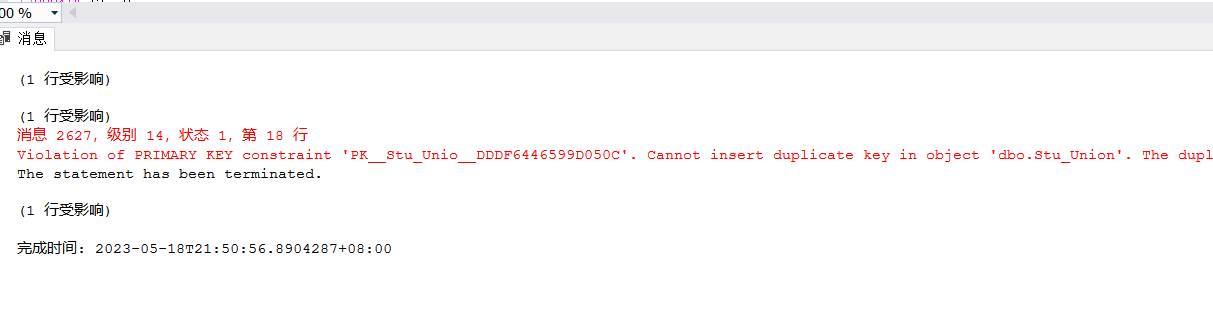
\includegraphics[width=0.6\textwidth]{1.png}
  \end{figure}

  \item 演示违反实体完整性的更新操作
  \inputminted[firstline=27,lastline=30]{sql}{../code/1.sql}

  \begin{figure}[H]
    \centering
    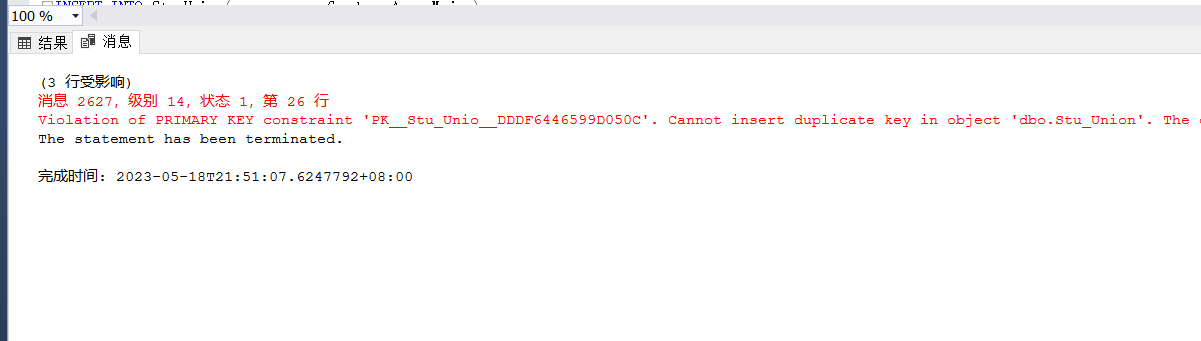
\includegraphics[width=0.6\textwidth]{2.png}
  \end{figure}

  \item 演示事务的处理,包括事务的建立,处理以及出错时的事物回滚
  \inputminted[firstline=35,lastline=43]{sql}{../code/1.sql}
  \begin{figure}[H]
    \centering
    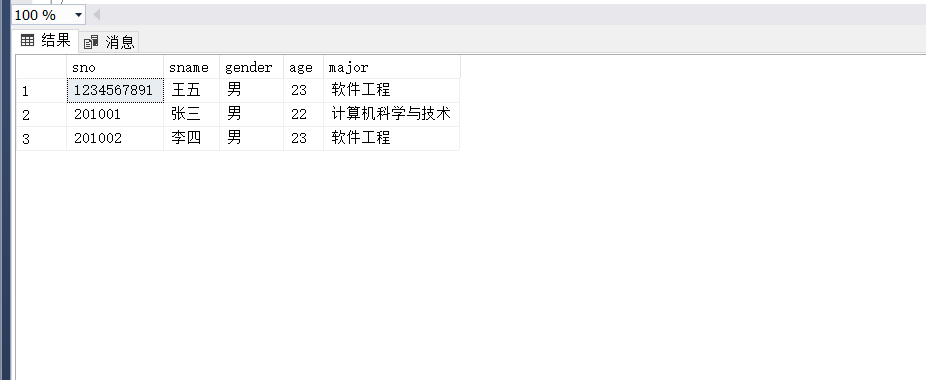
\includegraphics[width=0.6\textwidth]{3.png}
  \end{figure}
  \item 通过建立Scholarship表,插入一些数据。演示当与现有的数据环境不等时,无法建立实体完整性以及参照完整性。
  \inputminted[firstline=46,lastline=55]{sql}{../code/1.sql}
  \begin{figure}[H]
    \centering
    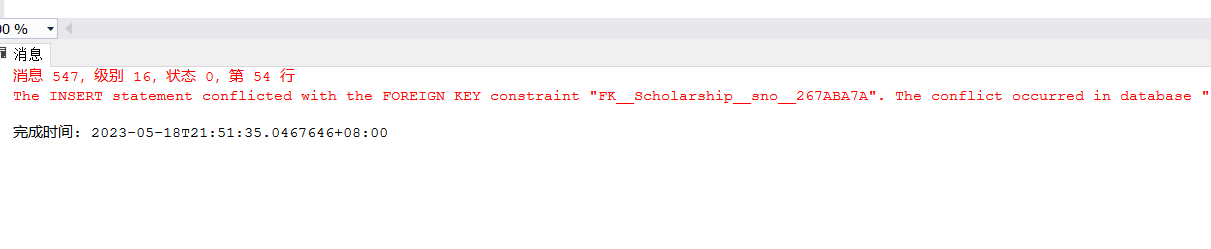
\includegraphics[width=0.6\textwidth]{4.png}
  \end{figure}
\end{enumerate}

\section{参照完整性}

\begin{enumerate}
\item 为演示参照完整性,建立表Course,令cno为其主键,并在Stu\_Union中插入数据。为下面的实验步骤做预先准备。
\inputminted[firstline=1,lastline=13]{sql}{../code/2.sql}
\item 建立表sc,另sno和cno分别为参照Stu\_Union表以及Course表的外键,设定为级连删除,并令(sno, cno)为其主键。在不违反参照完整性的前提下,插入数据。
\inputminted[firstline=14,lastline=28]{sql}{../code/2.sql}
\item 演示违反参照完整性的插入数据
\inputminted[firstline=31,lastline=32]{sql}{../code/2.sql}
\begin{figure}[H]
  \centering
  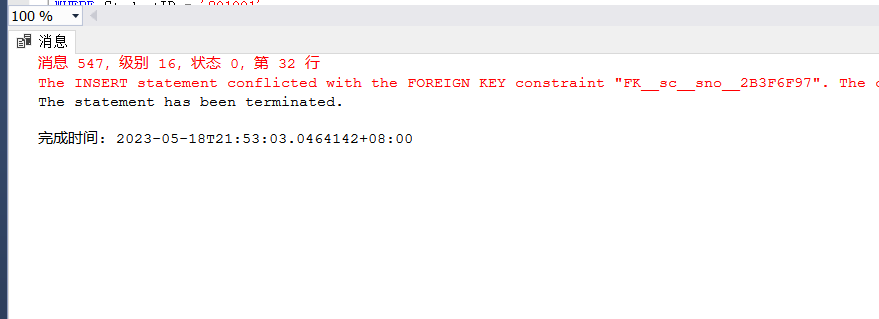
\includegraphics[width=0.6\textwidth]{5.png}
\end{figure}
\item 在Stu\_Union中删除数据,演示级连删除。
\inputminted[firstline=36,lastline=37]{sql}{../code/2.sql}
\begin{figure}[H]
  \centering
  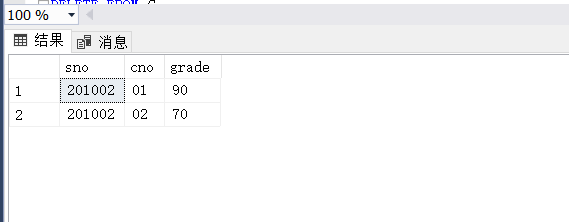
\includegraphics[width=0.6\textwidth]{6.png}
\end{figure}
\item Course中删除数据,演示级连删除。
\inputminted[firstline=42,lastline=44]{sql}{../code/2.sql}
\begin{figure}[H]
  \centering
  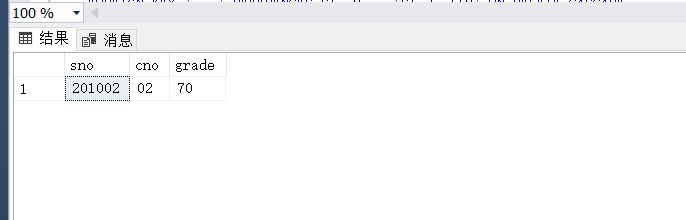
\includegraphics[width=0.6\textwidth]{7.png}
\end{figure}
\item 为了演示多重级连删除,建立Stu\_Card表,令stu\_id为参照Stu\_Union表的外键,令card\_id为其主键,并插入数据。
\inputminted[firstline=49,lastline=59]{sql}{../code/2.sql}
\item 为了演示多重级连删除,建立ICBC\_Card表,令stu\_card\_id为参照Stu\_Card表的外键,令bank\_id为其主键,并插入数据。
\inputminted[firstline=61,lastline=71]{sql}{../code/2.sql}
\begin{figure}[H]
  \centering
  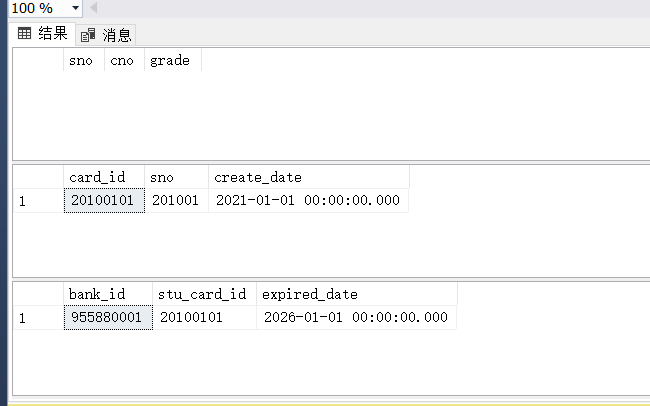
\includegraphics[width=0.6\textwidth]{8.png}
\end{figure}
\item 通过删除students表中的一条记录,演示三个表的多重级连删除。
\inputminted[firstline=74,lastline=79]{sql}{../code/2.sql}
\begin{figure}[H]
  \centering
  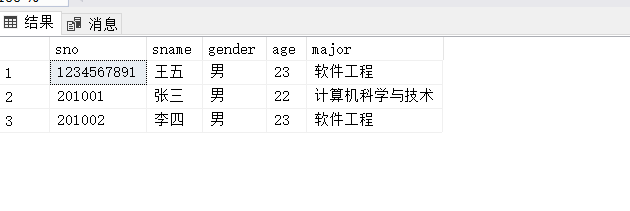
\includegraphics[width=0.6\textwidth]{9.png}
\end{figure}
\item 演示事务中进行多重级连删除失败的处理。修改ICBC\_Card表的外键属性,使其变为On delete No action, 演示事务中通过删除students表中的一条记录,多重级连删除失败,整个事务回滚到事务的初始状态。
\inputminted[firstline=82,lastline=100]{sql}{../code/2.sql}
\begin{figure}[H]
  \centering
  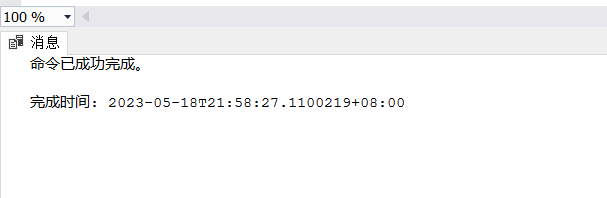
\includegraphics[width=0.6\textwidth]{10.png}
\end{figure}
\item 演示互参照问题及其解决方法。建立教师授课和课程指定教师听课关系的两张表,规定一个教师可以授多门课,但是只能去听一门课。为两张表建立相互之间的参照关系,暂时不考虑听课教师和授课教师是否相同(有余力的同学可以尝试限定听课与授课教师不相同)。
\inputminted[firstline=104,lastline=135]{sql}{../code/2.sql}
\end{enumerate}

\section{触发器的应用}

\begin{enumerate}
\item 在表sc中演示触发器的insert操作,当学生成绩低于60分时,自动改为60,并在事先创建的记录表中插入一条学生成绩低于60的记录。
\inputminted[firstline=1,lastline=30]{sql}{../code/3.sql}
\begin{figure}[H]
  \centering
  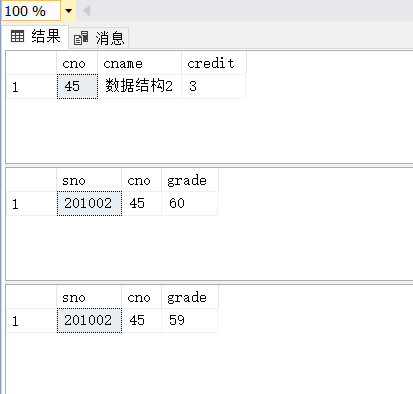
\includegraphics[width=0.4\textwidth]{11.png}
\end{figure}
\item 在表stu\_union中创建行级触发器,触发事件是UPDATE。当更新表stu\_union的Sid时,同时更新sc中的选课记录。
\item \begin{figure}[H]
  \centering
  \caption{修改前}
  \begin{subfigure}{0.45\textwidth}
  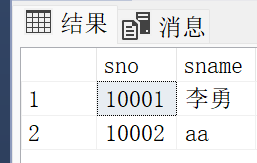
\includegraphics[width=0.6\textwidth]{133-1.png}
  \end{subfigure}
  \begin{subfigure}{0.45\textwidth}
    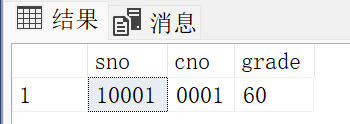
\includegraphics[width=0.6\textwidth]{133-2.png}
    \end{subfigure}
\end{figure}
\inputminted[firstline=42,lastline=54]{sql}{../code/3.sql}
\begin{figure}[H]
  \centering
  \caption{修改后}
  \begin{subfigure}{0.45\textwidth}
  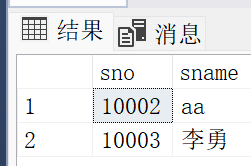
\includegraphics[width=0.6\textwidth]{133-3.png}
  \end{subfigure}
  \begin{subfigure}{0.45\textwidth}
    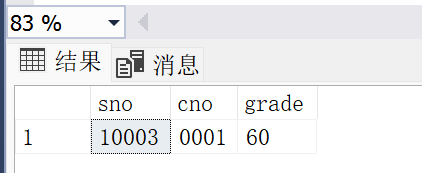
\includegraphics[width=0.6\textwidth]{133-4.png}
    \end{subfigure}
\end{figure}
\item 在表stu\_union中删除一学生的学号(演示触发器的delete 操作),使他在sc中关的信息同时被删除。
\begin{figure}[H]
  \centering
  \caption{修改前}
  \begin{subfigure}{0.45\textwidth}
  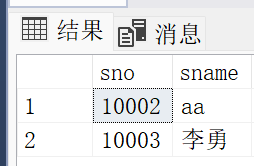
\includegraphics[width=0.6\textwidth]{134-1.png}
  \end{subfigure}
  \begin{subfigure}{0.45\textwidth}
    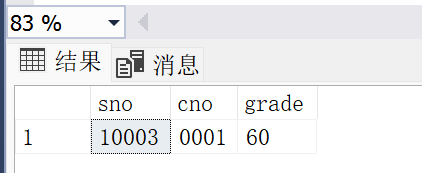
\includegraphics[width=0.6\textwidth]{134-2.png}
    \end{subfigure}
\end{figure}
\inputminted[firstline=58,lastline=70]{sql}{../code/3.sql}
\begin{figure}[H]
  \centering
  \caption{修改后}
  \begin{subfigure}{0.45\textwidth}
  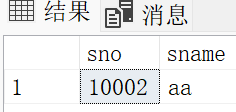
\includegraphics[width=0.6\textwidth]{134-3.png}
  \end{subfigure}
  \begin{subfigure}{0.45\textwidth}
    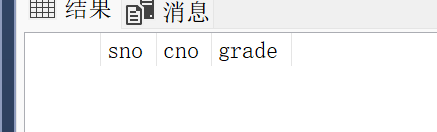
\includegraphics[width=0.6\textwidth]{134-4.png}
    \end{subfigure}
\end{figure}
\item 演示触发器删除操作。
\inputminted[firstline=74,lastline=76]{sql}{../code/3.sql}
\end{enumerate}

\section{索引的建立和作用}

\begin{enumerate}
\item STUDENTS(sid,sname,email,grade)在sname上建立聚簇索引,grade上建立非聚簇索引,并分析所遇到的问题
\inputminted[firstline=1,lastline=14]{sql}{../code/4.sql}

建立聚簇索引出错,因为默认为主键建立聚簇索引,要先删除主键的聚簇索引才能建索引。

\item 数据库SCHOOL的选课表CHOICES有如下结构:
CHOICES(no,sid,tid,cid,score)
假设选课表集中用于查询分析,经常执行统计某课程修读的学生人数查询访问
要求:
A.	首先执行没有索引的实验(设数据库CHOICES表在cid列上没有索引)
B.	然后做有索引的实验
C.	对比试验结果,并进行分析
\inputminted[firstline=17,lastline=34]{sql}{../code/4.sql}

\begin{figure}[H]
  \centering
  \begin{subfigure}{0.45\textwidth}
  \caption{没有索引}
  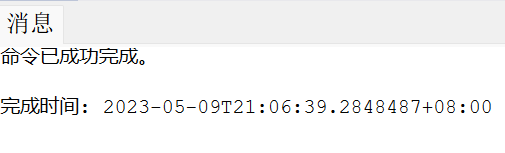
\includegraphics[width=0.6\textwidth]{142-1.png}
  \end{subfigure}
  \begin{subfigure}{0.45\textwidth}
  \caption{有索引}
    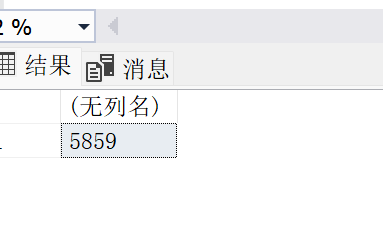
\includegraphics[width=0.6\textwidth]{142-2.png}
    \end{subfigure}
\end{figure}

使用索引可以显著提高查询性能,特别是当针对大型数据集进行查询时。
因此,在设计数据库时,为了优化查询性能,我们应该考虑添加恰当的索引来支持常见的查询操作。
例如,为经常使用的列添加索引,或者为经常连接的表添加外键索引,以提高查询的效率。 
然而,值得注意的是,过多的索引可能会对数据库性能产生负面影响。 
因此,在创建索引时必须在性能和查询效率之间找到平衡点。

\item 以数据库SCHOOL中CHOICES表为例,设建表时考虑到以后经常有一个用sid查询此学生所有选课信息的查询,考虑到一般学生不止选一门课,且要询问这些记录的所有信息,故在sid上建立索引,使相同sid的记录存在一起,取数据页面时能一起取出来,减少数据页面的存取次数
要求:
A.	首先执行没有任何索引的情况
B.	在sid上建有非聚簇索引的情况
C.	在sid上建有聚簇索引的情况
D.	对比实验结果,并进行分析


\begin{figure}[H]
  \centering
  \begin{subfigure}{0.45\textwidth}
  \caption{没有索引}
  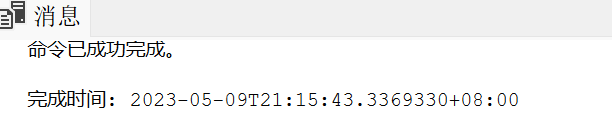
\includegraphics[width=0.6\textwidth]{143-1.png}
  \end{subfigure}
  \begin{subfigure}{0.45\textwidth}
  \caption{有非聚簇索引}
    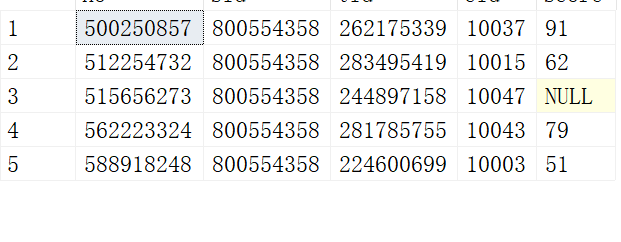
\includegraphics[width=0.6\textwidth]{143-2.png}
  \end{subfigure}
  \begin{subfigure}{0.45\textwidth}
    \caption{有聚簇索引}
      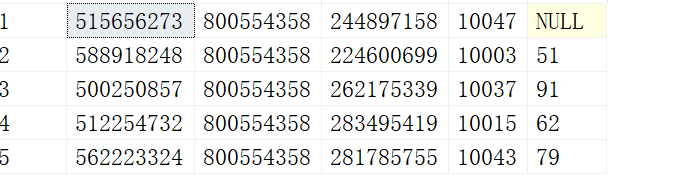
\includegraphics[width=0.6\textwidth]{143-3.png}
    \end{subfigure}
\end{figure}

\inputminted[firstline=38,lastline=45]{sql}{../code/4.sql}

通过比对实验结果并进行分析,可以得出以下结论:
\begin{enumerate}
\item 在没有索引的情况下,每次查询都需要扫描整个表,效率较低,随着数据量的增加,查询语句的执行时间会逐渐变长。因此,在表的大小较大时,没有索引会显著影响查询性能。
\item 使用聚集索引进行查询时,它首先找到符合查询条件的第一条记录,然后根据索引中定义的列值顺序去查找下一条记录,直到找到满足所有查询条件的所有记录为止。由于聚簇索引是按照行的物理存储顺序排列的,因此查询时磁盘的读取次数会减少,从而提高查询速度。
\item 使用非聚簇索引进行查询时,它首先根据索引列的值查找对应的记录,然后使用指针定位实际行数据,最后返回符合查询条件的结果。与聚簇索引不同,使用非聚簇索引进行查询时需要进行额外的磁盘读取,因此查询速度可能会受到一定的影响。
\end{enumerate}

\end{enumerate}

\section{实验总结}

在本次实验中,我了解了实体完整性并学会了如何定义主键以保证唯一性。更好地理解实体与关系型表的关系
我还了解了参照完整性以及如何用外键约束实现关系型表之间数据的一致性,学会了触发器的基本原理和用处。
实际操作了通过触发器对表中的数据进行限制和管理的方法,练习了编写触发器所需的语法。
同时,对不同的索引进行了对比,更好地理解了相关的知识。

\end{spacing}

\end{document}